
%%%%%%%%%%%%%%%%%%%%%%% file typeinst.tex %%%%%%%%%%%%%%%%%%%%%%%%%
%
% This is the LaTeX source for the instructions to authors using
% the LaTeX document class 'llncs.cls' for contributions to
% the Lecture Notes in Computer Sciences series.
% http://www.springer.com/lncs       Springer Heidelberg 2006/05/04
%
% It may be used as a template for your own input - copy it
% to a new file with a new name and use it as the basis
% for your article.
%
% NB: the document class 'llncs' has its own and detailed documentation, see
% ftp://ftp.springer.de/data/pubftp/pub/tex/latex/llncs/latex2e/llncsdoc.pdf
%
%%%%%%%%%%%%%%%%%%%%%%%%%%%%%%%%%%%%%%%%%%%%%%%%%%%%%%%%%%%%%%%%%%%


\documentclass[runningheads,a4paper]{llncs}

\usepackage{amssymb}
\usepackage{amsmath}
\setcounter{tocdepth}{3}
\usepackage{graphicx}
\usepackage{algorithm}
\usepackage[noend]{algorithmic}


\usepackage{url}


\begin{document}

\mainmatter  % start of an individual contribution

% first the title is needed
\title{A Post-Quantum Digital Signature Scheme \\ based on Supersingular Isogenies}

% a short form should be given in case it is too long for the running head
%\titlerunning{Lecture Notes in Computer Science: Authors' Instructions}

% the name(s) of the author(s) follow(s) next
%
% NB: Chinese authors should write their first names(s) in front of
% their surnames. This ensures that the names appear correctly in
% the running heads and the author index.
%
\author{Reza Azarderakhsh \and David Jao \and Youngho Yoo}
%
%\authorrunning{Lecture Notes in Computer Science: Authors' Instructions}
% (feature abused for this document to repeat the title also on left hand pages)

% the affiliations are given next; don't give your e-mail address
% unless you accept that it will be published
\institute{University of Waterloo}

%
% NB: a more complex sample for affiliations and the mapping to the
% corresponding authors can be found in the file "llncs.dem"
% (search for the string "\mainmatter" where a contribution starts).
% "llncs.dem" accompanies the document class "llncs.cls".
%

\toctitle{Lecture Notes in Computer Science}
\tocauthor{Authors' Instructions}
\maketitle


\begin{abstract}
We present the first digital signature scheme based on supersingular elliptic curve isogenies. The signature is secure against quantum adversaries, has small key sizes, and can take advantage of offline computation to sign efficiently. We also provide various implementation results. This scheme is an application of Unruh's construction of non-interactive zero-knowledge proofs to an interactive zero-knowledge proof proposed by De Feo and Jao.
\keywords{Digital signatures, Isogenies, Post-quantum cryptography}
\end{abstract}



\section{Introduction}

Quantum computers can efficiently solve certain classically intractable problems such as integer factoring and finding discrete logarithms. The hardness of these problems forms the foundation of the security of most public-key cryptosystems in use today. Thus, quantum computers pose a serious threat to modern cryptography. Post-quantum cryptography is the study of classical cryptosystems that remain secure against quantum computers.  There are several candidates for post-quantum cryptographic primitives, such as those based on lattices, codes, or hashes. One based on supersingular elliptic curve isogenies was proposed by De Feo, Jao, and Pl\^ut \cite{FJP14}, who gave protocols for key establishment, zero-knowledge proof of identity, and public key encryption. The key establishment protocol has seen various efficient implementations \cite{Costello16,AKJKJ16}, and the zero-knowledge proof can be implemented by a slight modification to the key establishment protocol.

Additional care must be taken when discussing the security of post-quantum cryptosystems. A proof of security requires a reduction from an adversary breaking the cryptosystem to an efficient algorithm solving the underlying problem, and in some cases classical proofs no longer work against quantum adversaries. The standard Fiat-Shamir transform \cite{FS87} for turning a zero-knowledge proof of knowledge into a digital signature scheme is such an example. The classical security proof of Fiat-Shamir uses a technique called \emph{rewinding}, where we observe the adversary's output, then rewind the adversary back to some previous saved state during its execution. We then reprogram the random oracle so that the adversary will produce a different output when run again, and use the two different outputs to solve the problem.

In the quantum setting, we cannot copy and save an adversary state, due to the no-cloning theorem \cite{WZ82}. Moreover, if we tried to rewind the adversary by applying an inverse transformation to its initial output, then measuring the output would disturb the adversary's state. In some restricted cases quantum rewinding is possible \cite{Watrous09,Unruh12}, but it remains hard in the general case. It has also been shown that the Fiat-Shamir transform is in general not quantum-secure, relative to a specific oracle \cite{ARU14}.

Another issue is that of the quantum random oracle. The random oracle model allows us to use ideal random functions for security proofs, but in a real world implementation they must be replaced by cryptographically secure hash functions. Then it seems restrictive to only allow classical queries to the hash function, since many implementations will use a known and well-established hash function, which a quantum adversary can implement on its own and query in superposition. In other words, we must allow the adversary the query the random oracle in superposition. This makes it difficult to reprogram the random oracle, since it is impossible to exactly determine the query input when it is in superposition.

Unruh \cite{Unruh15} proposed a transformation with a property called \emph{online extractability} which allows us to extract the witness (private key) from a successful adversary without rewinding. It also avoids the problem of determining the query inputs by including the output values of query inputs which we want to learn. We apply this construction to the zero-knowledge proof of De Feo and Jao to obtain a digital signature scheme secure against quantum adversaries in the quantum random oracle model, and provide implementation results.



\subsection*{Our Contributions}
\begin{itemize}
	\item We construct the first digital signature scheme based on supersingular elliptic curve isogenies. Our scheme achieves very small key sizes and, with offline precomputation, is able to sign messages extremely quickly. It is the first application of Unruh's transformation for constructing signatures, and it is strongly unforgeable under chosen message attack (SUF-CMA) against quantum adversaries in the quantum random oracle model.
	 
	\item We provide implementation results on computers as well as on embedded devices with optimized arithmetic.
\end{itemize}








\section{Unruh's construction}

We fix a binary relation $R$. A statement $x$ holds if there exists $w$ such that $(x,w) \in R$. In this case, we call $w$ a \emph{witness} to $x$. In a proof system, a prover $P$ tries to prove a statement $x$ to a verifier $V$ (in other words, $P$ tries to convince $V$ that $P$ knows a witness $w$). We assume that all parties have access to a quantum random oracle $H$ which can be queried in superposition.

\subsection{Non-interactive proofs}
A non-interactive proof system consists of two polynomial time algorithms, a prover $P(x,w)$ outputting a proof $\pi$ of the statement $x$, and a verifier $V(x,\pi)$ outputting whether or not it accepts the proof $\pi$ of $x$.

Let $(P,V)$ be a non-interactive proof system. We define the following properties:
\begin{itemize}
	\item 
	{\bf Completeness:} If $(x,w) \in R$, then $V$ accepts the proof $\pi = P(x,w)$ with overwhelming probability.

	\item
	{\bf Zero-knowledge (NIZK):} There is a polynomial time simulator $S$ such that, given the ability to program the random oracle, $S$ can output proofs indisinguishable by any quantum polynomial time algorithm from those produced by $P$. 

	The simulator is modeled as two algorithms $S = (S_{init}, S_P)$, where $S_{init}$ outputs an initial circuit $H$ simulating a random oracle, and $S_P$ produces proofs using $H$. $S_P$ is a stateful algorithm which may modify or replace $H$ with a different oracle.

	\item
	{\bf Simulation-sound online-extractability} (with respect to simulator $S = (S_{init}, S_P)$): There is a polynomial time algorithm (extractor) $E$ such that, for all quantum algorithms $A$ with quantum access to a simulated random oracle $H \leftarrow S_{init}$ and classical access to the prover $S_P$, if $A$ outputs a new valid proof of a statement $x$, then $E$ can compute a witness $w$ such that $(x,w) \in R$.
\end{itemize}



\subsection{Sigma protocols} 
A \emph{sigma protocol} is an interactive proof system in which a prover $P=(P^1,P^2)$ tries to prove a statement $x$ to a verifier $V$. Sigma protocols consist of three messages in order: the commitment $com = P^1(x,w)$ made by the prover, the challenge $ch$ chosen uniformly at random by the verifier, and the response $resp = P^2(x,w,com,ch)$ computed by the prover based on the challenge. Then $V$ outputs $V(x,com,ch,resp) \in \{0,1\}$, indicating whether or not they accept the proof.

Let $\Sigma$ be a sigma protocol. We define the following properties:
\begin{itemize}
	\item
	{\bf Completeness:} If $P$ knows a witness $w$ to the statement $x$, then $V$ always accepts.

	\item
	{\bf Computational special soundness:} There is a polynomial time extractor $E_\Sigma$ such that, given any valid interactions $(com,ch,resp)$ and $(com, ch', resp')$ that $V$ accepts, where $ch \neq ch'$, $E_\Sigma$ can compute a witness $w$ such that $(x,w) \in R$ with overwhelming probability.

	\item
	{\bf Honest-verifier zero-knowledge (HVZK):} There is a polynomial time simulator $S_\Sigma$ with outputs of the form $(com, ch, resp)$ that is indistinguishable from valid interactions between an honest prover and verifier by any quantum polynomial time algorithm.

\end{itemize}

\subsection{The transformation}
Unruh's construction transforms a complete sigma protocol with special soundness and HVZK into a complete NIZK proof with simulation-sound online extractability. Suppose we have a sigma protocol $\Sigma = (P_\Sigma^1, P_\Sigma^2, V_\Sigma)$, where there are $c$ possible challenges in the challenge domain $N_{ch}$ and the parties want to run the protocol $t$ times.  Then we define a non-interactive proof system $(P_{OE}, V_{OE})$ as follows.

\begin{algorithm}
\caption{Prover: $P_{OE}$ on input $(x,w)$}
\begin{algorithmic}
\STATE $\texttt{// Create $t\cdot c$ proofs and hash each response}$
\FOR {$i=1\ \TO\ t$} 
	\STATE $com_i \leftarrow P_\Sigma^1(x,w)$
	\FOR {$j=1\ \TO\ c$}
		\STATE $ch_{i,j} \leftarrow_R N_{ch} \setminus \{ch_{i,1},\dots,ch_{i,j-1}\}$
		\STATE $resp_{i,j} \leftarrow P_\Sigma^2(x,w,com_i, ch_{i,j})$
		\STATE $h_{i,j} \leftarrow G(resp_{i,j})$
	\ENDFOR
\ENDFOR
\vspace{2mm}
\STATE $\texttt{// Get challenge by hashing}$
\STATE $J_1 \| \dots \| J_t \leftarrow H(x, (com_i)_i, (ch_{i,j})_{i,j}, (h_{i,j})_{i,j})$ 
\vspace{2mm}
\STATE \texttt{// Return proof}
\RETURN {$\pi \leftarrow ((com_i)_i, (ch_{i,j})_{i,j}, (h_{i,j})_{i,j}, (resp_{i,J_i})_i) $}
\end{algorithmic}
\end{algorithm}

\begin{algorithm}
\caption{Verifier: $V_{OE}$ on input $(x,\pi)$, where \newline $\pi = ((com_i)_i, (ch_{i,j})_{i,j}, (h_{i,j})_{i,j}, (resp_{i,J_i})_i)$}
\begin{algorithmic}
\STATE $\texttt{// Compute the challenge hash}$
\STATE $J_1 \| \dots \| J_t \leftarrow H(x, (com_i)_i, (ch_{i,j})_{i,j}, (h_{i,j})_{i,j})$ 
\vspace{2mm}
\FOR {$i=1\ \TO\ t$}
	\STATE {\bf check} $ch_{i,1},\dots,ch_{i,m}$ pairwise distinct
	\STATE {\bf check} $h_{i,J_i} = G(resp_i)$
	\STATE {\bf check} $V_\Sigma(x,com_i, ch_{i,J_i}, resp_i) = 1$
\ENDFOR
\IF {all checks succeed}
	\RETURN 1
\ENDIF
\end{algorithmic}
\end{algorithm}

\begin{theorem}[Corollary 19 in \cite{Unruh15}]
If $\,\Sigma$ satisfies completeness, special soundness, and HVZK, then $(P_{OE}, V_{OE})$ is a complete non-interactive zero-knowledge proof system with simulation-sound online extractability.
\end{theorem}

\subsection{Signatures}
A \emph{digital signature} scheme consists of three algorithms:
\begin{itemize}
	\item 
	$keygen(\lambda)$: takes a security parameter $\lambda$ and outputs a public-private key pair $(pk,sk)$.

	\item
	$sign(sk, m)$: takes the private key $sk$ and signs the message $m$, outputting a signature $\sigma$.

	\item
	$ver(pk, m, \sigma)$: takes the public key of the claimed signer and verifies the signature $\sigma$ on the message $m$.
\end{itemize}

A digital signature $\mathcal{S} = (keygen, sign, ver)$ is \emph{strongly unforgeable under chosen message attack (SUF-CMA)} if, for any quantum polynomial time adversary $A$ with classical access to the signing oracle $sig: m \mapsto sign(sk,m)$, $A$ cannot produce a new valid message-signature pair with non-negligible probability.


Suppose we have a key generator outputting $(pk,sk)$ such that the problem of computing $sk$ from $pk$ is hard (for quantum polynomial time algorithms), and let $(P,V)$ be a NIZK proof of knowledge of the secret key. To obtain a signature scheme, we just need to incorporate the message $m$ that is being signed. We do this by including the message in the statement so that statements have the form $x = (pk,m)$ (the witness is the private key), and the message is incorporated into the challenge hash: $J_1 \| \dots \| J_t \leftarrow H(pk,m,(com_i)_i, (ch_{i,j})_{i,j}, (h_{i,j})_{i,j})$. 

To sign a message, we simply run $\sigma \leftarrow P(x,w)$. To verify the signature, we run $V(x,\sigma)$ and output the result.

Unruh shows that a signature scheme obtained this way is secure, as long as it is difficult to compute $sk$.

\begin{theorem}[\cite{Unruh15}]
If $(P,V)$ is a complete NIZK proof with simulation-sound online extractability, then the above signature scheme is SUF-CMA.
\end{theorem}
\begin{proof}[Proof (outline).]
Let $A$ be a quantum polynomial time adversary capable of forging a new message-signature pair with access to random oracle $H$ and a classical signing oracle $sig$. Since $(P,V)$ is zero-knowledge, we can simulate $H$ and $sig$, indistinguishable to $A$. Then when $A$ outputs a new message-signature pair, by simulation-sound online extractability, we can efficiently extract the witness, thereby obtaining the secret key.
\end{proof}










\section{Isogeny-based signature}
\subsection{Preliminaries}
An \emph{isogeny} is a rational map between elliptic curves that preserves the point at infinity. Isogenies are necessarily group homomorphisms and can be identified with their kernels, thus there is a one-to-one correspondence between isogenies and subgroups of the curve. The degree of an isogeny is its degree as a rational map, and is equal to the size of its kernel. Two curves $E_1$ and $E_2$ are isogenous over $\mathbb{F}_q$ if and only if $\#E_1(\mathbb{F}_q) = \#E_2(\mathbb{F}_q)$ [ref]. Every isogeny $\phi: E_1 \to E_2$ of degree $d$ has a unique dual isogeny $\hat \phi:E_2 \to E_1$ (which can be computed efficiently) of the same degree such that $\hat \phi \circ \phi : E_1 \to E_1$ is the multiplication map $P \mapsto [d]P$.

The set of isogenies mapping a curve $E$ to itself forms a ring, called the endomorphism ring, under pointwise addition and composition. A curve $E$ is \emph{supersingular} if its endomorphism ring is isomorphic to an order in a quaternion algebra, and \emph{ordinary} otherwise. All supersingular elliptic curves over finite fields of characteristic $p$ are defined over $\mathbb{F}_{p^2}$.

The $\ell$-torsion group of $E$ is defined as $E[\ell] = \{P \in E(\overline{\mathbb{F}}_{p^2}) : [\ell] P = \mathcal{O}\}$. If $p \nmid \ell$, then $E[\ell] \cong (\mathbb{Z}/\ell\mathbb{Z})^2$.

\subsection{Zero-knowledge proof of identity}
We use primes of the form $p = \ell_A^{e_A}\ell_B^{e_B}f \pm 1$ where $\ell_A, \ell_B$ are small primes (typically 2 and 3) and $f$ is a small cofactor to ensure $p$ is prime. Then it is easy to construct a supersingular curve $E(\mathbb{F}_{p^2})$ of order $(\ell_A^{e_A}\ell_B^{e_B}f)^2$ [ref].

The setup for the zero-knowledge proof of identity is as follows. There is a public curve $E$ of order $(\ell_A^{e_A}\ell_B^{e_B}f)^2$ and public generators $P_B, Q_B$ of $\ell_B^{e_B}$-torsion group $E[\ell_B^{e_B}] = \langle P_B,Q_B\rangle$. Peggy (the prover) has a secret point $S$ of order $\ell_A^{e_A}$ generating a secret subgroup $\langle S \rangle$, defining an isogeny $\phi:E \to E/\langle S\rangle$ of degree $\ell_A^{e_A}$. She publishes $E/\langle S \rangle$ as well as $\phi(P_B), \phi(Q_B)$, the images of the public generators under her secret isogeny.

To choose a random secret point $S$, Peggy chooses generators $P_A,Q_A$ of $E[\ell_A^{e_A}]$, and chooses random $m_A,n_A \in \mathbb{Z}/\ell_A^{e_A}\mathbb{Z}$ such that $m_A,n_A$ are not both divisible by $\ell_A$. She then computes the random point $S := [m_A]P_A + [n_A]Q_A$.

\ifx %%%%%%%%%%%%%%%%%%%%%%%%%%%%%%%%%%%%%%%%%%%%%%%%%%%%%%%
\begin{figure}[ht]\label{FigZKP}
\centering
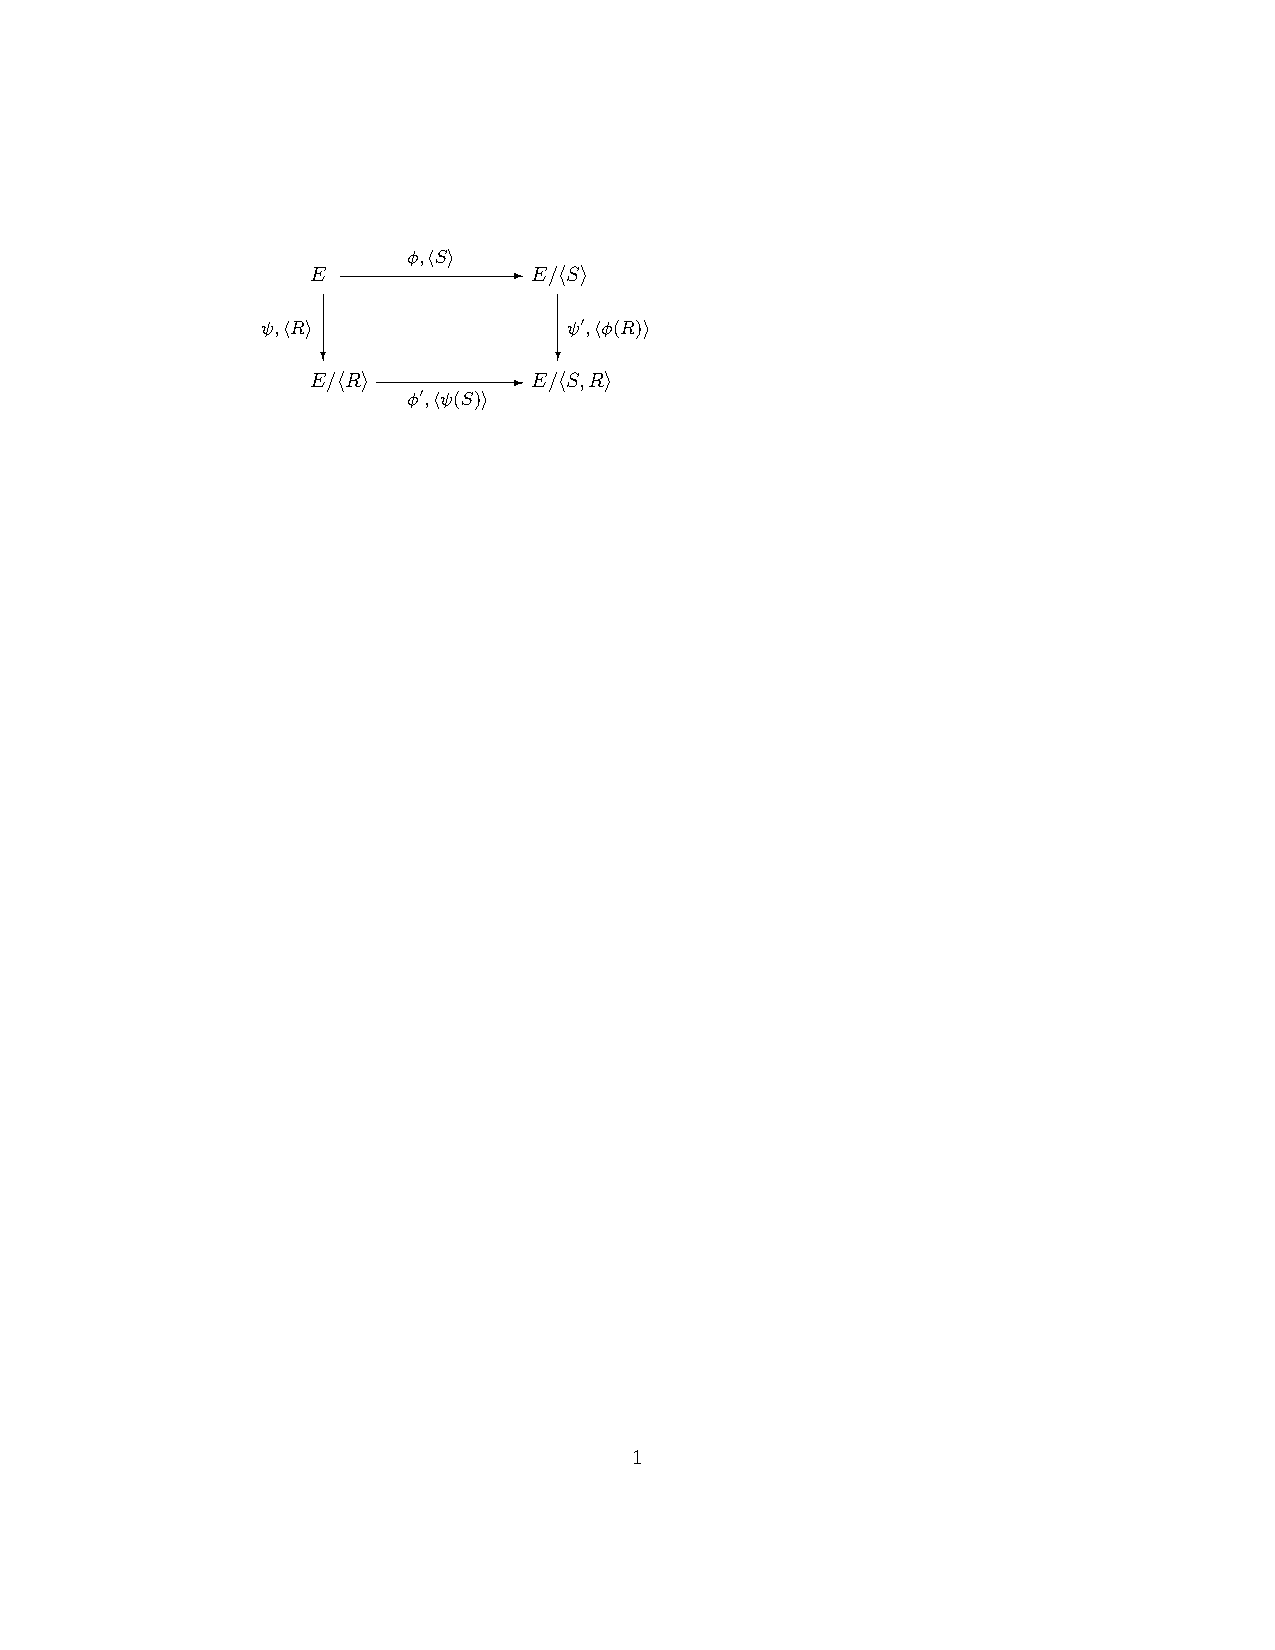
\includegraphics[trim= 120 595 300 120, clip=true]{zkpdiagram.pdf}
\begin{center} \caption{Each arrow is labelled by the isogeny and its kernel}
\end{center}
\end{figure}
\fi

For Peggy to identify herself to Vic (the verifier), they run the following protocol:
\begin{enumerate}
	\item 
	\begin{itemize}
		\item Peggy chooses a random point $R$ of order $\ell_B^{e_B}$ by choosing random $m_B,n_B$ not both divisible by $\ell_B$.

		\item She computes the isogeny $\psi: E \to E/\langle R \rangle$. 

		\item She then computes the isogeny $\phi':E/\langle R \rangle \to E/\langle R,S\rangle$ with kernel $\langle\psi(S)\rangle$ (alternatively $\psi':E/\langle S \rangle \to E/\langle R,S\rangle$ with kernel $\langle\phi(R)\rangle$)

		\item She sends the commitment $(E_1,E_2)$ to Vic, where $E_1 = E/\langle R \rangle$ and $E_2 = E/\langle R,S\rangle$.
	\end{itemize}

	\vspace{2mm}

	\item
	Vic randomly chooses a challenge bit $b \in \{0,1\}$ and sends it to Peggy.

	\vspace{2mm}
	
	\item
	\begin{itemize}
		\item If $b=0$, Peggy sends the response $(R,\phi(R))$.
		\item If $b=1$, Peggy sends the response $\psi(S)$.
	\end{itemize}

	\vspace{2mm}
	
	\item
	\begin{itemize}
		\item If $b=0$, Vic verifies that $R$ and $\phi(R)$ have order $\ell_B^{e_B}$ and generate the kernels for the isogenies $E \to E_1$ and $E/\langle S \rangle \to E_2$ respectively.
		
		\item If $b=1$, Vic verifies that $\psi(S)$ has order $\ell_A^{e_A}$ and generates the kernel for the isogeny $E_1 \to E_2$.
	\end{itemize}
\end{enumerate}

This sigma protocol is complete, due to the fact that the diagram in \ref{FigZKP} commutes. It also satisfies computational zero-knowledge and special soundness assuming the following problems (from \cite{FJP14}) are hard.

\begin{problem}[Computational Supersingular Isogeny (CSSI) problem]
Let $\phi_A:E_0 \to E_A$ be an isogeny whose kernel is $\langle R_A \rangle$ where $R_A$ is a random point with order $\ell_A^{e_A}$. Given $E_A, \phi_A(P_B), \phi_A(Q_B)$, find a generator of $\langle R_A \rangle$.
\end{problem}

\begin{problem}[Decisional Supersingular Product (DSSP) problem]
Let $\phi:E_0 \to E_3$ be an isogeny of degree $\ell_A^{e_A}$ and let $(E_1,E_2,\phi')$ be sampled with probability 1/2 from the following distributions:
\begin{itemize}
	\item 
	A random point $R$ of order $\ell_B^{e_B}$ is chosen and $E_1 = E_0/\langle R \rangle$, $E_2 = E_3/\langle \phi(R) \rangle$, and $\phi':E_1 \to E_2$ is an isogeny of degree $\ell_A^{e_A}$.

	\item
	$E_1$ is chosen randomly among curves of the same cardinality as $E_0$, and $\phi':E_1 \to E_2$ is a random isogeny of degree $\ell_A^{e_A}$
\end{itemize}
Determine which of the two distributions $(E_1,E_2,\phi')$ was sampled.
\end{problem}

\begin{theorem} [\cite{FJP14}]
The ZKP protocol satisfies HVZK and special soundness.
\end{theorem}
\begin{proof}
To prove HVZK, we construct a simulator as follows. First choose a random bit $b \in \{0,1\}$. 

If $b=0$, then we choose random $R$ and output $(com,ch,resp)$ where $com = (E/\langle R\rangle, E/\langle R,S\rangle)$, $ch = b = 0$, and $resp = (R,\phi(R))$.

If $b=1$, then we choose a random supersingular curve $E'$ with cardinality $(\ell_A^{e_A}\ell_B^{e_B}f)^2$, and a random point $S'$ of order $\ell_A^{e_A}$. We output $(com,ch,resp)$ where $com = (E', E'/\langle S' \rangle)$, $ch=b=1$, and $resp = S'$. This is indistinguishable from a valid execution of the protocol to any quantum polynomial-time adversary under the assumption that the DSSP problem is hard.

To prove special soundness, suppose we have two valid transcripts $(com,0,resp_0)$ and $(com,1,resp_1)$, where $com = (E_1,E_2)$. Parse $resp_0$ as $(R,\phi(R))$ and $resp_1$ as $\psi(S)$ and compute $\phi:E \to E/\langle R \rangle$. Then we can compute the dual isogeny $\hat \phi:E/\langle R \rangle$, and $\hat\phi(\psi(S))$ is a generator for $\langle S \rangle$.
\end{proof}

The best known attack for the CSSI problem takes $O(p^{1/6})$ time. Thus, to achieve security level $\lambda$, we use a prime with bitlength $6\lambda$.



\subsection{Signature}
Applying Unruh's construction to the zero-knowledge proof of identity, we obtain a digital signature scheme that is SUF-CMA. A description of the algorithms $(keygen,sign,ver)$ are give below.

\vspace{2mm}
{\bf Public Parameters:} Security parameter $\lambda$, a prime $p = \ell_A^{e_A}\ell_B^{e_B}f \pm 1$ of bitlength $6\lambda$, a supersingular curve $E$ over $\mathbb{F}_{p^2}$ of cardinality $(p \mp 1)^2 = (\ell_A^{e_A}\ell_B^{e_B})^2$, and generators $(P_B,Q_B)$ of the torsion group $E[\ell_B^{e_B}]$.

\begin{algorithm}[ht]
\caption{$keygen(\lambda)$}
\begin{algorithmic}
\STATE{Pick a random point $S$ of order $\ell_A^{e_A}$}
\STATE{Compute the isogeny $\phi:E \to E/\langle S \rangle$}
\STATE{$pk \leftarrow (E/\langle S \rangle, \phi(P_B), \phi(Q_B))$}
\STATE{$sk \leftarrow S$}
\RETURN $(pk,sk)$
\end{algorithmic}
\end{algorithm}

\begin{algorithm}[ht]
\caption{$sign(sk,m)$}
\begin{algorithmic}
\FOR {$i=1\ \TO\ 2\lambda$}
	\STATE {Pick a random point $R$ of order $\ell_B^{e_B}$}
	\STATE {Compute the isogeny $\psi:E \to E/\langle R \rangle$}
	\STATE {$E_1 \leftarrow E/\langle R \rangle$}
	\STATE {$E_2 \leftarrow E/\langle R,S\rangle$} 
	\STATE $com_i \leftarrow (E_1,E_2)$
	\STATE {$ch_i \leftarrow_R \{0,1\}$}
	\STATE $resp_{i,0} \leftarrow (R,\phi(R))$
	\STATE $resp_{i,1} \leftarrow \psi(S)$
	\IF {$ch_i = 1$}
		\STATE $swap(resp_{i,0},resp_{i,1})$
	\ENDIF
	\STATE $h_{i,j} \leftarrow G(resp_{i,j})$
\ENDFOR
\vspace{2mm}
\STATE $J_1 \| \dots \| J_{2\lambda} \leftarrow H(pk,m, (com_i)_i, (ch_{i,j})_{i,j}, (h_{i,j})_{i,j})$ 
\vspace{2mm}
\RETURN {$\sigma \leftarrow ((com_i)_i, (ch_{i,j})_{i,j}, (h_{i,j})_{i,j}, (resp_{i,J_i})_i) $}
\end{algorithmic}
\end{algorithm}

\begin{algorithm}[ht]
\caption{$ver(pk,m, \sigma)$}
\begin{algorithmic}
\STATE $J_1 \| \dots \| J_{2\lambda} \leftarrow H(m,x, (com_i)_i, (ch_{i,j})_{i,j}, (h_{i,j})_{i,j})$ 
\vspace{2mm}
\FOR {$i=1\ \TO\ 2\lambda$}
	\STATE {\bf check} $h_{i,J_i} = G(resp_{i,J_i})$
	\IF {$ch_i = 0$}
		\STATE Parse $(R,\phi(R))\leftarrow resp_{i,J_i}$
		\STATE {\bf check} $R,\phi(R)$ have order $\ell_B^{e_B}$
		\STATE {\bf check} $R$ generates the kernel of the isogeny $E \to E_1$
		\STATE {\bf check} $\phi(R)$ generates the kernel of the isogeny $E/\langle S \rangle \to E_2$
	\ELSE
		\STATE Parse $\psi(S) \leftarrow resp_{i,J_i}$
		\STATE {\bf check} $\psi(S)$ has order $\ell_A^{e_A}$
		\STATE {\bf check} $\psi(S)$ generates the kernel of the isogeny $E_1 \to E_2$ 
	\ENDIF
\ENDFOR
\IF {all checks succeed}
	\RETURN 1
\ENDIF
\end{algorithmic}
\end{algorithm}

Note that, to achieve $\lambda$ bits of security, the protocol must be run $2\lambda$ times, since a quantum adversary can choose arbitrary bits $J_1 \| \dots \| J_t$ to compute simulated proofs based on those bits, then perform a pre-image search on $H$ using Grover's algorithm \cite{Grover96} to find a message $m$ that will give the required hash.





\subsection{Implementation}
We implemented the signature scheme by modifying the Supersingular Isogeny Diffie-Hellman (SIDH) library published by Costello, Longa, and Naehrig \cite{Costello16}. We describe some implementation details. For full details, refer to \cite{FJP14,Costello16}.

The SIDH implementation uses a fixed prime and initial curve
\begin{align*}
p &= 2^{372}\cdot 3^{239}-1 \\
E_0\!\!&\ : y^2 = x^3+x
\end{align*}
The prime $p$ has bitlength 751, thus each field element requires 1502 bits. It provides 186 bits of classical security and 124 bits of quantum security. The curve $E_0$ is a supersingular curve with order $(p+1)^2 = (2^{372}\cdot 3^{239})^2$.

The performance of the SIDH library is summarized in the table \cite{Costello16}. Alice and Bob each have a secret point $R_A,R_B$ of orders $2^{372}, 3^{239}$ respectively.
Alice's (resp. Bob's) keygen operation computes the isogeny $\phi_A:E_0 \to E_A= E/\langle R_A\rangle$ (resp. $\phi_B:E_0 \to E_B= E/\langle R_B \rangle$). Then the shared key operation computes $\phi_A':E_B \to E_B / \langle \phi_B(R_A)\rangle$ (resp. $\phi_B': E_A \to E_A/ \langle \phi_A(R_B)\rangle$). This gives them the shared secret $E_{AB} = E/\langle R_A,R_B\rangle$. 

\begin{table}[ht]
\centering
\begin{tabular}{l|l|l}
Operation			&	Sandy Bridge	&	Haswell \\ \hline
Alice's keygen		&	50				&	46		\\
Bob's keygen		&	57				&	52		\\
Alice's shared key 	&	47				&	44		\\
Bob's shared key 	&	55 				&	50		
\end{tabular}
\caption{Performance results of the SIDH library given in \cite{Costello16}, expressed in millions of clock cycles, taken on a 3.4GHz Intel Core i7-2600 Sandy Bridge and a 3.4GHz Intel Core i7-4770 Haswell processor.}
\end{table}

Note that computing degree $2^{372}$ isogenies is faster than degree $3^{239}$ isogenies in both keygen and shared key operations.
In the signature scheme, we repeatedly execute the zero-knowledge proof (see Figure \ref{FigZKP}), computing $\psi$ and one of $\phi'$, $\psi'$ for each round of the ZKP protocol. So to reduce signing time, we switched $A$ and $B$ in our implementation. In other words, we use $\ell_A^{e_A} = 3^{239}$ and $\ell_B^{e_B} = 2^{372}$ so that $\psi,\psi'$ are degree $2^{372}$ isogenies, and always use $\psi'$ to compute $E/\langle R,S\rangle$ when signing.

With the switch, the public generators for the torsion groups are:
\begin{align*}
P_A &= [2^{372}](6, \sqrt{6^3+6}) 	& Q_A = \varphi(P_A)	&& \\
P_B &= [3^{239}](11,\sqrt{11^3+11}) 	& Q_B = \varphi(P_B) &&
\end{align*}
where $E[3^{239}] = \langle P_A,Q_A\rangle$ and $E[2^{372}] = \langle P_B, Q_B\rangle$,
and $\varphi: (x,y) \mapsto (-x,iy)$ is the distortion map (where $i = \sqrt{-1}$) [ref].

To sample random points of order $3^{239}$, we randomly choose $n' \in \{1,\dots, 3^{238}-1\}$ and set $S = P_A + [3n']Q_A$. Then $S$ has order $3^{239}$ [ref]. Each $n'$ generates a distinct subgroup, so this samples from a set of $3^{239}-1$ subgroups. Note that there are $4\cdot 3^{239}$ cyclic subgroups of order $3^{239}$, so we are only sampling from about 1/4 of all possible isogenies of degree $3^{239}$. This does not seem to have an immediate impact on security, and reduces the private key size to $\lceil \log_2 3^{238} \rceil = 378$ bits.

Similarly, to sample random points of order $2^{372}$, we randomly choose $n' \in \{1,\dots,2^{372}-1\}$ and compute $R = P_B + [2n']Q_B$. This samples from a set of $2^{372}-1$ subgroups out of $3\cdot 2^{372}$ possible subgroups. 

Isogenies of degree $\ell^e$ can be computed by composing $e$ isogenies of degree $\ell$. See \cite{FJP14,Costello16} for detailed analysis on optimizing isogeny computations.

The SIDH implmentation uses projective coordinates for both points and curve coefficients to reduce the number of field inversions. The curves that we use are isomorphic to Montgomery curves which have the form $E_{(a,b)}: by^2 = x^3+ax^2+x$. The Kummer line on a Montgomery curve, which identifies each point $(X:Y:Z)$ with its inverse $(X:-Y:Z)$, allows us to disregard the $Y$ coordinate and has efficient arithmetic. This allows us to represent points by just one field element $X/Z$ in $\mathbb{F}_{p^2}$. We can still add two points $P,Q$ by \emph{differential addition} if we know the $x$-value of $P-Q$. Isogeny computations are unaffected because a point $P$ and its inverse $-P$ generate the same subgroup.  

Similarly, we can ignore the $b$ coordinate of the Montgomery curve coefficients, as it turns out that there are only two ismorphism classes of Montgomery curves for a given coefficient value $a$, and they have the same Kummer line. Thus, curves can also be represented by one field element.




\subsubsection{Sizes}
As mentioned above, the private key can be stored using 378 bits, or 48 bytes. The public key contains the curve $E/\langle S \rangle$, the $x$ coordinates of the images of the generators $\phi(P_B),\phi(Q_B)$, and $\phi(P_B-Q_B)$ for differential addition. Each can be represented using one field element, so the total size of the public key is $4 \cdot 1502 = 6008$ bits, or 751 bytes.

The signature contains $(com_i, ch_{i,0}, h_{i,1-J_i}, resp_{i,J_i})$ for each round $i$ of the ZKP protocol. The commitment has two curves, $com_i=(E_1,E_2)$, requiring two field elements, or 3004 bits. The challenge $ch_{i,0}$ requires just 1 bit, and $ch_{i,1}$ can be inferred from $ch_{i,0}$. The verifier can compute $h_{i,J_i} = G(resp_{i,J_i})$, so it may be omitted. $h_{i,1-J_i}$ should be a 248-bit hash for 124-bit quantum security. 

The response can have varying length depending on the challenge bit $J_i$. If $J_i = 0$, then the response should contain $R,\phi(R)$, but it suffices to send the coefficient $n'$ where $R = P_B + [2n']Q_B$. Then the verifier can compute $R$ and $\phi(R) = \phi(P_B)+[2n']\phi(Q_B)$. So if $J_i=0$, then 371 bits suffice. If $J_i=1$, then we must send the $x$ coordinate of $\psi(S)$, requiring 1502 bits.

Thus for each ZKP round, the signature requires on average $3004 + 1 + 248 + (371+1502)/2 = 4189.5$ bits. For quantum 124 bit security, we require 248 rounds, so the expected signature size is $248 \cdot 4189.5 = 1038996$ bits, or 129875 bytes.


\subsubsection{Performance}
Performance tests were run on an Intel Xeon E5-2637 v3 3.5 GHz Haswell processor. Note that the signing and verifying algorithms are easily parallelizable with linear speedup, since the computations required for each round of the ZKP protocol is independent. These computation results are summarized below.  

\begin{table}[ht]
\centering
\begin{tabular}{c | c c c c}
threads	&	keygen 	& 	signing   	& verifying \\ \hline
1		&	63	     	& 	28776   	& 19679     \\ 
2		&	-		&	14474	& 10042	\\
4		&	-		&	7449		& 5536	\\
8		&	-		&	5537		& 3953	
\end{tabular}
\caption{Performance results (in $10^6$ CPU clock cycles) on Intel Xeon E5-2637 v3 3.5 GHz.}
\end{table}

We have also implemented the signature on an ARM Cortex-A57 in both C and ASM, with an optimized arithmetic library on the latter. The optimized arithmetic gives significant improvement in performance over the C implementation based on the SIDH library, as shown below.

\begin{table}[ht]
\centering
\begin{tabular}{c | c | c}
Operation		&	C		& 	ASM	\\ \hline
ZKP Avg.		&	2,999		&	222 	\\
Ver. round Avg. &	1,928		&	143	\\ \hline
Key gen		&	1,656		&	123	\\
Signature		&	767,928	&	57,092	\\
Verification	&	493,797	&	36,757
\end{tabular}
\caption{Performance results (in $10^6$ CPU clock cycles) on ARM Cortex-A57}
\end{table}




\bibliographystyle{splncs03}

\bibliography{bibliography}




\end{document}
